\documentclass[11pt,english]{article}
\usepackage[T1]{fontenc}
\usepackage[latin9]{inputenc}
\usepackage{babel}
\usepackage{verbatim}
\usepackage{float}
\usepackage{amsmath}
\usepackage{amssymb}
\usepackage{setspace}
\usepackage{graphicx}
\usepackage{subfigure}
\usepackage{pdfpages}

\PassOptionsToPackage{normalem}{ulem}
\usepackage{ulem}
\onehalfspacing
%\usepackage[unicode=true,pdfusetitle,
% bookmarks=true,bookmarksnumbered=false,bookmarksopen=false,
% breaklinks=false,pdfborder={0 0 1},backref=section,colorlinks=false]
% {hyperref}
\usepackage{hyperref}
%\usepackage{breakurl}


%%%%%%%%%%%%%%%%%%%%%%%%%%%%%% User specified LaTeX commands.

\usepackage{latexsym}
\addtolength{\hoffset}{-0.75in}
\addtolength{\voffset}{-0.75in}
\addtolength{\textwidth}{1.5in}
\addtolength{\textheight}{1.6in}

%\usepackage{Sweave}
%\include{Sweave}
%\usepackage{listings}

% === dcolumn package ===
\usepackage{dcolumn}\newcolumntype{.}{D{.}{.}{-1}}
\newcolumntype{d}[1]{D{.}{.}{#1}}

\usepackage{comment}

% === more new math commands
\newcommand{\X}{\mathbf{X}}
\newcommand{\Y}{\mathbf{Y}}
\renewcommand{\r}{\right}
\renewcommand{\l}{\left}
\newcommand{\dist}{\buildrel\rm d\over\sim}
\newcommand{\ind}{\stackrel{\rm indep.}{\sim}}
\newcommand{\ud}{\mathrm{d}}
\newcommand{\iid}{\stackrel{\rm i.i.d.}{\sim}}
\newcommand{\logit}{{\rm logit}}
\newcommand{\cA}{\mathcal{A}}
\newcommand{\E}{\mathbb{E}}
\newcommand{\V}{\mathbb{V}}
\newcommand{\cJ}{\mathcal{J}}
\newcommand{\bone}{\mathbf{1}}
\newcommand{\var}{{\rm Var}}
\newcommand{\cov}{{\rm Cov}}
\newcommand{\tomega}{\tilde\omega}

% === spacing
\newcommand{\spacingset}[1]{\renewcommand{\baselinestretch}%
{#1}\small\normalsize}
% \spacingset{1.2}
\setlength{\parindent}{0pt}
\setlength{\parskip}{2em}
%%%%%%%%%%%%%%%%%%%%%%%%%%%%%%%%%%%%%%%%%%%%%%%%%%%%%%%%%%%%%%%%%%%%%%%%%%%%%%%

\begin{document}

1) $\X = (X_{(1)}, X_{(2)}, \ldots, X_{(m)})$ is orthogonal, so $X_{(i)}^t X_{(j)} = 0$ for $i \neq j$ and 1 for $i = j$. \\
$tr(\mathbf{P}) = tr(\X \X^t) = tr(\X^t \X) = tr\left( (X_{(i)}^t X_{(j)})_{i,j} \right) = tr(I_{m*m}) = m$ \par


2) Since $A$ is symmetric, $A = KDK^t$, where is $K$ is orthogonal and D is the diagonal matrix with elements, $d_1, \ldots, d_n$.\\
$\because \displaystyle\lim_{k \rightarrow \infty} KA^kK^t = K(\displaystyle\lim_{k \rightarrow \infty}A^k)K^t $and $K$ is orthogonal.\\
$\therefore \displaystyle\lim_{k \rightarrow \infty} KA^kK^t =0 \Leftrightarrow \displaystyle\lim_{k \rightarrow \infty} A^k=0$
\begin{flalign*}
&\displaystyle\lim_{k \rightarrow \infty} KA^kK^t = \displaystyle\lim_{k \rightarrow \infty} (KAK^t)^k = \displaystyle\lim_{k \rightarrow \infty} D^t =0&\\
&\Leftrightarrow \lim d_i^k = 0 \qquad i=1,\ldots,n \Leftrightarrow |d_i| < 1 \qquad i=1,\ldots,n &\\
&\therefore \displaystyle\lim_{k \rightarrow \infty} A^k=0 \Leftrightarrow |d_i| < 1 \qquad i=1,\ldots,n &
\end{flalign*}
\par

3)(a)\begin{flalign*}
&\forall x \in \mathbb{R}^n &\\
&x^t(A-C)x = x^t(A-B)x + x^t(B-C)x&\\
&\because x^t(A-B)x > 0 \text{ and } x^t(B-C)x>0 \qquad \text{since} A\rhd B, B \rhd C&\\
&x^t(A-C)x > 0 \Rightarrow A \rhd C&
\end{flalign*}
(b)
\begin{flalign*}
&\because A\rhd B \text{ and } B \rhd A&\\
&\forall x \in \mathbb{R}^n, \quad x^t(A-B)x \geq 0 \text{ and } x^t(B-A)x \geq 0&\\
&\Rightarrow x^t(A-B)x=0 \quad \forall x \in \mathbb{R}^n \Rightarrow A=B&
\end{flalign*}
\par


4)(a)Let $A = SS^t$ and $B=UU^t$ are the Cholesky decomposition.  Then $A^{-1} = S^{-t}S^{-1}$ and $B^{-1} = U^{-t}U^{-1}$.\\
 Assume $x^tBx = 1$, then $x^tAx \geq 1$ since $A\rhd B$.  This means at the minimum point, the term is still true.  So differentiae $x^tAx - \lambda (x^tBx -1)$, we get:\\
$$ Ax = \lambda Bx, \Rightarrow x^tAx = \lambda x^tBx = \lambda$$
According to lecture2 page 122, $\lambda y = U^{-1}AU^{-t}y = U^{-1}SS^{t}U^{-t}y$, where eigenvalue $\lambda \geq 1$.\\
For $x^tA^{-1}x = 1$, now we calculate the minimum value of $x^tB^{-1}x$.  Then $\mu y = (S^{-t})^{-1}B^{-1}(S^{-t})^{-t} y = S^{t}U^{-t}U^{-1}S y $.  Note $S^{t}U^{-t}U^{-1}S$ and $U^{-1}AU^{-t} = U^{-1}SS^{t}U^{-t}$ have the same eigenvalues (AB and BA have the same eigenvalues).  So eigenvalue $\mu \geq 1 \quad \forall \mu$. Thus $x^tB^{-1}x - x^tA^{-1}x \geq 0$, namely $ B^{-1} \rhd A^{-1}$.\\
(b) In the notation of (a), $U^{-1}SS^{t}U^{-t}$ and $SS^{t}U^{-t}U^{-1} = AB^{-1}$ have the same eigenvalues.  Thus $det(AB^{-1})=det(U^{-1}SS^{t}U^{-t}) \geq 1 \Rightarrow det(A) \geq det(B)$. \\
$C = A-B$ is a semi-positive definite matrix and suppose $\exists i,\quad c_{ii} < 0 $.  Let $x = e_i$, then $x^t(A-B)x < 0$, which contradicts the condition.  So $\forall i, \quad c_{ii} \geq 0 \Rightarrow tr(A-B) \geq 0 \Rightarrow tr(A) \ge tr(B)$.\par

5) For multivariate Gaussian, $M_{\X}(t) = e^{\mu^t t} + \frac{1}{2}t^t\Sigma t$.  For univariate Gaussian, $M_X(t) = e^{\mu t+ \frac{1}{2}\sigma^2t}$.  Distributions and moment generating functions are one-to-one map.\\
$\Rightarrow$     $\forall k \in \mathbb{R}, \alpha \in \mathbb{R}^n, \quad   M_{\X}(k\alpha) = \E e^{k\alpha^t\X} =  e^{\mu^t\alpha k + \frac{1}{2}(\alpha^t \Sigma \alpha)k^2} = M_{\alpha^t\X}(k)$.  So $\forall \alpha,\quad \alpha^t\X\sim N(\mu^t\alpha, \alpha^t \Sigma \alpha) $\\
$\Leftarrow$     $\forall t \in \mathbb{R}^n,\quad M_{t^t\X}(1) = e^{t^t\mu + \frac{1}{2}t^t\Sigma t} = M_{\X}(t)$  So $\X \sim N_{\X}(\mu, \Sigma)$\par


6)Let A be a $n*n$ positive definite.  A = $\begin{pmatrix}
                                             A_{11} & A_{12}\\
                                             A_{21} & A_{22}
                                           \end{pmatrix}$, where $A_{11}$ is a $m*m$ ($m < n$) matrix.\\
Let $x_{1*m}$ be nonzero and $y = (x_{1*m}^t, 0^t_{1*(n-m)})^t$, then $y^tAy = x^tA_{11}x > 0$. Thus, $A_{11}$ is positive definite. So is $A_{22}$ in similar method.  When $m=1$, $a_{11} = A_{11} > 0$.  And $A_{22}$ is positive definite, so its element in first row and first column, $a_{22}$ is greater than 0.  Apply the above method to $A_{22}$.  In this way ,we get $a_{ii}>0, \quad i=1,\ldots, n$.\\
Let $a = (\sqrt{a_{11}}, \frac{a_{12}}{\sqrt{a_{11}}}, \ldots, \frac{a_{1n}}{\sqrt{a_{11}}})^t$, $A_{12}=(a_{12}, \ldots, a_{1n})$ and $A_{21} = A^t_{12}$.  Then,
\begin{flalign*}
&A - aa^t=
\left(
\begin{array}{@{\,}c|ccc@{\,}}
0&0&\dots&0\\
\hline
0&&&\\
\vdots &\multicolumn{3}{c}{\raisebox{-10pt}[0pt][0pt]{\Huge $A'$}}\\
0&&&\\
0&&&\\
\end{array}
\right) &\\
&\text{where, } A' = A_{22} - A_{21}a_{11}^{-1}A_{12}&
\end{flalign*}
Let $ y = (-\frac{A_{12}}{a_{11}}x, x^t)^t$, where $x \in \mathbb{R}^{n-1}$, then $y^tAy = x^t (A_{22}-A_{21}a^{-1}_{11}A_{12}) x > 0$. So $A_{22}-A_{21}a^{-1}_{11}A_{12}$ is positive definite.  Then we could apply the same method to $A_{22}-A_{21}a^{-1}_{11}A_{12}$.  In this way, we construct a upper triangular matrix $T$ such that $A = T^tT$.\\
Suppose there are two upper triangular matrices $T$ and $S$, which satisfy Cholesky decomposition.  \\
1. Since $T^tT = S^tS = A$, then $t_{11}^2 = s_{11}^2 = a_{11}$.  Then $t_{11} = s_{11} > 0$.\\
2. $\because t_{11}t_{1i} = s_{11}s_{1i} = a_{1i} \therefore t_{1i} = s_{1i}, \quad i = 2,\ldots, n$ \\
3. $\because t_{12}^2 + t_{22}^2 = s_{12}^2 + s_{22}^2 \therefore t_{22} = s_{22} > 0 $\\
4. keep applying the same technique until $t_{nn} = s_{nn} >0$.\\
So $T=S$. \par

7)
\begin{flalign*}
&q_1 = \frac{v_1}{\| v_1 \|} = (0.2822163, 0.5644325, 0.7525767, 0.1881442)&\\
&q_2 = \frac{v_2 - <v_2, q_1>q_1}{\| v_2 - <v_2, q_1>q_1 \|} = (0.6531533, -0.6473902,  0.1498410,  0.3630764)&\\
&q_3 = \frac{v_3 - <v_3, q_1>q_1 - <v_3, q_2>q_2}{\| v_3 - <v_3, q_1>q_1 - <v_3, q_2>q_2 \|} = (0.45151564, -0.02620403,  0.07256501, -0.88892142)&
\end{flalign*}\par


8)
\begin{flalign*}
&\frac{1}{\sqrt{2}}
\left(
  \begin{array}{cc}
    V & V \\
    U & -U \\
  \end{array}
\right)
\left(
  \begin{array}{cc}
    D & 0 \\
    0 & -D \\
  \end{array}
\right)
\frac{1}{\sqrt{2}}
\left(
  \begin{array}{cc}
    V^t & U^t \\
    V^t & -U^t \\
  \end{array}
\right)
=%%%%%%%%%%%%%%%%%%%
\frac{1}{2}
\left(
  \begin{array}{cc}
    VD & -VD \\
    UD & UD \\
  \end{array}
\right)
\left(
  \begin{array}{cc}
    V^t & U^t \\
    V^t & -U^t \\
  \end{array}
\right)
&\\%%%%%%%%%%%%%%%%
&=\frac{1}{2}
\left(
  \begin{array}{cc}
    0 & 2VDU^t \\
    2UDV^t & 0 \\
  \end{array}
\right)
=
\left(
  \begin{array}{cc}
    0 & A^t \\
    A & 0 \\
  \end{array}
\right)&
\end{flalign*}

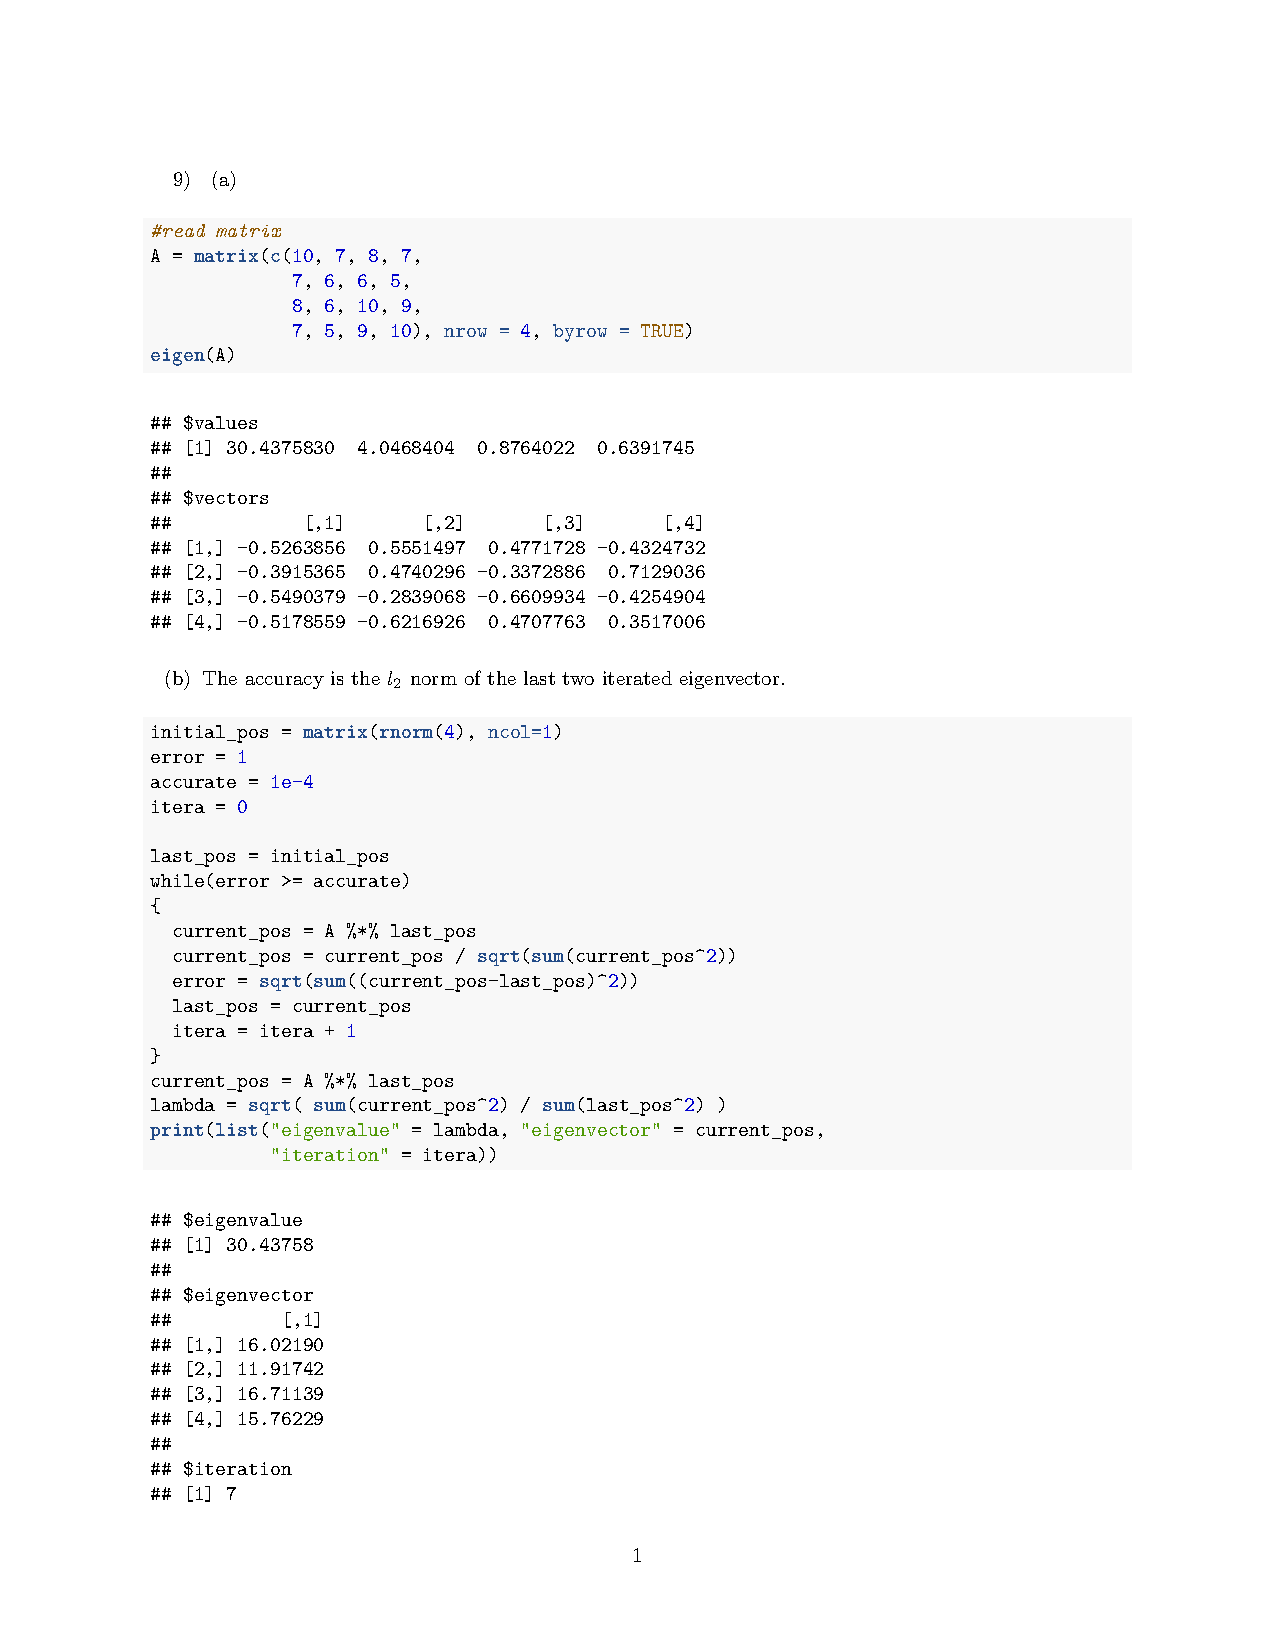
\includepdf[pages={1,2}]{hw2_last_question.pdf}





























\end{document}
